\documentclass[aspectratio=169]{beamer}

\usepackage[utf8]{inputenc}
%\usepackage{latexsym}
\usepackage{graphicx}
\usepackage{mathptmx}
\usepackage{amsmath}
%\usepackage{amsfonts}
\usepackage{amssymb}
\usepackage{amsbsy}
\usepackage{amsthm}
\usepackage{algorithmic}

% Get checkmark logo
\usepackage{pifont}
\newcommand{\cmark}{\ding{51}}
\newcommand{\xmark}{\ding{55}}
% Get \lee and \gee commands
\newcommand{\lee}{\leqq}
\newcommand{\gee}{\geqq}

% Strikouts
\usepackage[normalem]{ulem}

% Restore Mathcal
\let\saveboldmath\boldmath
\usepackage{mathptmx}
\let\boldmath\saveboldmath
\usepackage{bm}
\DeclareSymbolFont{cmsymbols}{OMS}{cmsy}{m}{n}
\SetSymbolFont{cmsymbols}{bold}{OMS}{cmsy}{b}{n}
\DeclareSymbolFontAlphabet{\mathcal}{cmsymbols}

\usepackage[english]{babel}
\usepackage[utf8]{inputenc}

% AMSLaTeX packages
\usepackage{amsthm}
\usepackage{amsmath}
\usepackage{amsfonts}
\usepackage[algoruled]{algorithm2e}

\usetheme{default}
\useoutertheme{default}
% we want to use images
\usepackage{graphicx}
\usepackage{movie15}
\usepackage{hyperref}

% table relates packages
\usepackage{booktabs}
\usepackage{multirow}
% pick a font
\usepackage{palatino}           
% \usepackage{times}
\usepackage{tikz}
\usetikzlibrary[positioning,arrows,decorations.pathmorphing,backgrounds,fit,calc]
% \AtBeginSection[]  % "Beamer, do the following at the start of every section"
% {
%   \begin{frame}<beamer> 
%     \frametitle{Outline} % make a frame titled "Outline"
%     \tableofcontents[currentsection]  % show TOC and highlight current section
%   \end{frame}                    
% }

% \AtBeginSubsection[]
% {
%   \begin{frame}
%     \frametitle{Outline}
%     \tableofcontents[currentsection,currentsubsection]
%   \end{frame}
% }

\AtBeginSection[]
{
   \begin{frame}
       \frametitle{Outline}
       \tableofcontents[currentsection]
   \end{frame}
}

\newcommand{\ebox}[1][1em]{\framebox[#1]{\phantom{M}}}

\setlength\arraycolsep{1.4pt}% some length

%gets rid of navigation symbols
\setbeamertemplate{navigation symbols}{}

%gets rid of bottom navigation bars
\setbeamertemplate{footline}[page number]{}
\setbeamertemplate{headline}{}


\usebackgroundtemplate{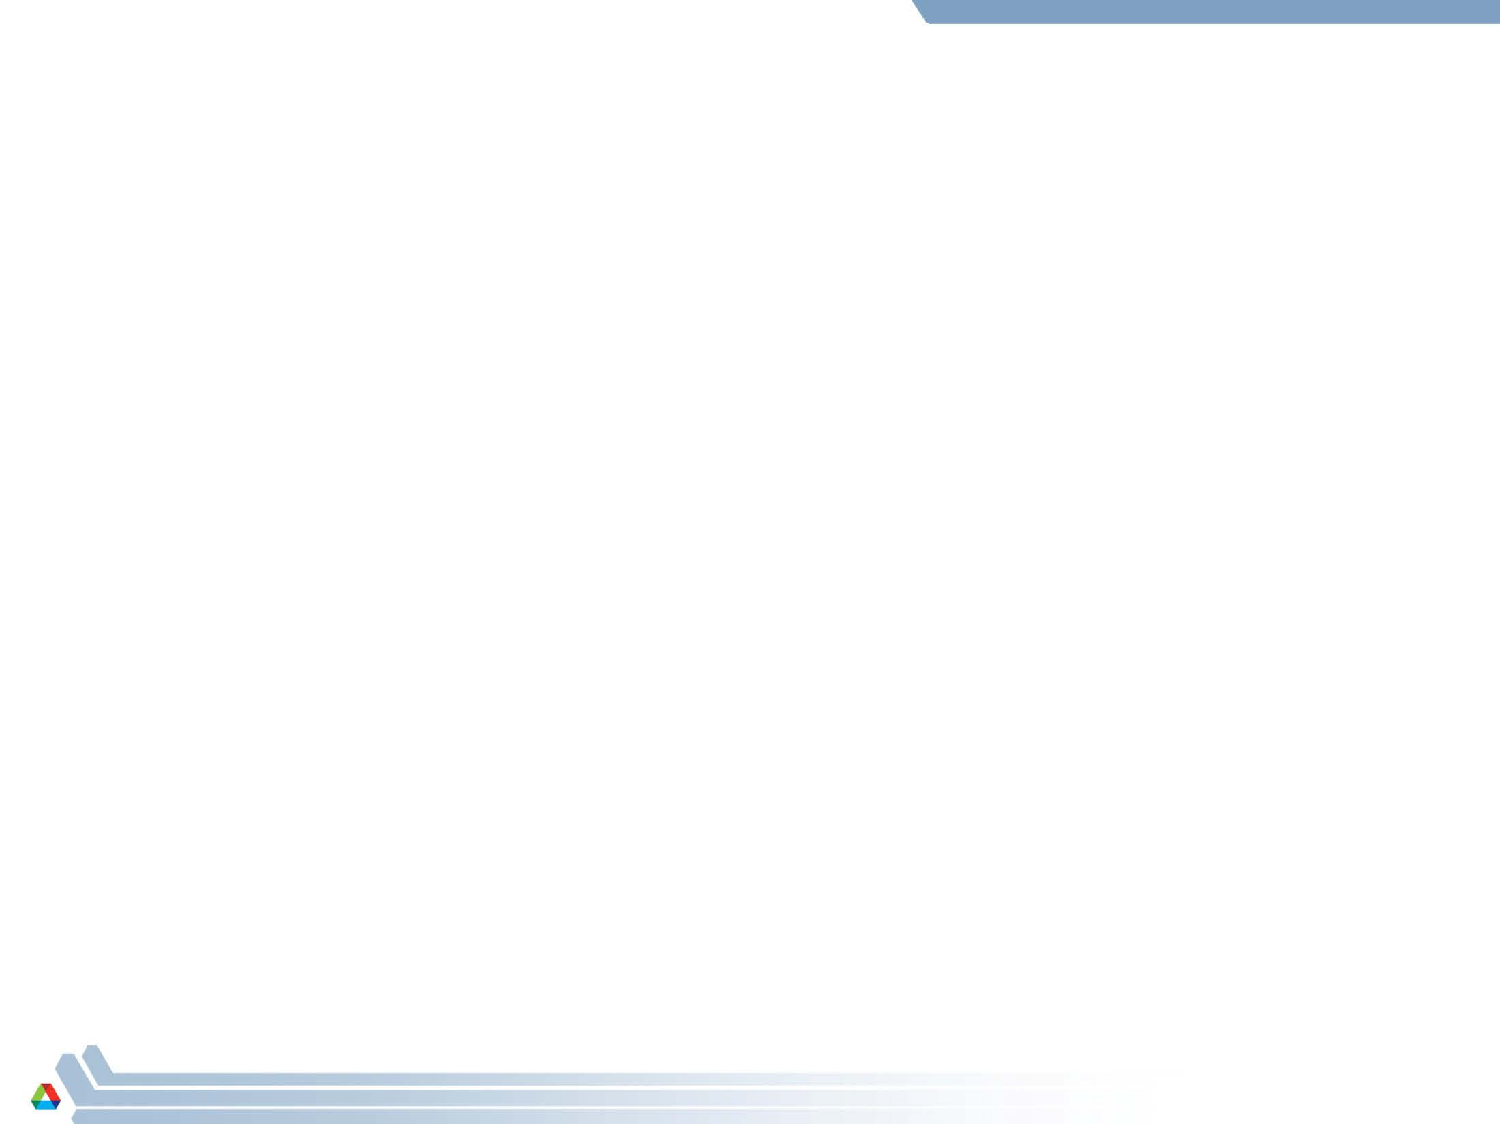
\includegraphics[width=\paperwidth]{../templates/NormalANLBlue}}
% Title Information
\title{Data sampling for surrogate modeling and optimization}
\author{Tyler Chang\\
(and others)}
\date{ICIAM 2023, Tokyo, Japan\\
Aug 23, 2023}
\institute{Argonne National Laboratory}

\begin{document}

\setbeamertemplate{footline}{}
{
\usebackgroundtemplate{
\includegraphics[width=\paperwidth]{../templates/TitleANLBlue}}
\frame{\titlepage}
}

\setbeamertemplate{footline}[page number]{}

% FRAME: overview
\begin{frame}
  \frametitle{Outlines}
  \tableofcontents
\end{frame}

\section{Inference problems and high-dimensional modeling}

\begin{frame}\frametitle{The fundamental machine learning problem}

\begin{columns}
\begin{column}{0.5\textwidth}

\onslide<2>{
\begin{center}
\includegraphics[width=\textwidth]{../img/delaunay_new/inference_1d_pt1.eps}
\end{center}
}

\onslide<3>{
\begin{center}
\vskip -14.5em
\includegraphics[width=\textwidth]{../img/delaunay_new/inference_1d_pt2.eps}
\end{center}
}

\onslide<4>{
\begin{center}
\vskip -14.5em
\includegraphics[width=\textwidth]{../img/delaunay_new/inference_1d_pt3.eps}
\end{center}
}

\onslide<5>{
\begin{center}
\vskip -14.5em
\includegraphics[width=\textwidth]{../img/delaunay_new/inference_1d_pt4.eps}
\end{center}
}

\onslide<6>{
\begin{center}
\vskip -14.5em
\includegraphics[width=\textwidth]{../img/delaunay_new/inference_1d_pt5.eps}
\end{center}
}

\end{column}
\begin{column}{0.5\textwidth}
\begin{itemize}
\onslide<2->{\item Want to predict unknown $f(x)$ for observation $x$}
\onslide<3->{\item {\bf ML}: {\sl Learn} approximation ${\hat f} \sim f$ based on {\sl training data} ${\cal X}$}
\onslide<3->{\item {\bf NA}: fit an interpolant (piecewise-linear) to $f$ on ${\cal X}$}
\onslide<4->{\item Both cases: more data $\Rightarrow$ better ${\hat f}$}
\onslide<5->{\item Real data not perfectly balanced  $\Rightarrow$ ${\hat f} \rightarrow f$ non-uniformly}
\onslide<6->{\item If we have enough data, it doesn't matter}
\end{itemize}
\end{column}
\end{columns}

\end{frame}

\begin{frame}
\frametitle{Some basic numerical analysis results}

\begin{columns}
\begin{column}{0.5\textwidth}
When ${\hat f}$ is a piecewise linear spline:

\bigskip

For $h$ ``small enough'' -- let $q$ be the querry point
$$
|f(q) - {\hat f}(q)| \sim {\cal O}( h^2)
$$
\end{column}
\begin{column}{0.5\textwidth}
\onslide<1>{
\begin{center}
\includegraphics[width=\textwidth]{../img/delaunay_new/inference_1d_pt5.eps}
\end{center}
}

\onslide<2>{
\begin{center}
\vskip -14.5em
\includegraphics[width=\textwidth]{../img/delaunay_new/inference_1d_pt2.eps}
\end{center}
}

\end{column}
\end{columns}
\begin{itemize}
\item $h$ is a ``mesh fineness'' parameter $\sim$ distance between points in ${\cal X}$
\item For irregular ${\cal X}$, $h$ could be the distance from $q$ to the nearest neighbor in ${\cal X}$
\item Constants proportional to the Lip constant of $\nabla f$
\end{itemize}
\end{frame}

\begin{frame}
\frametitle{Some basic deep learning}
\begin{columns}
\begin{column}{0.5\textwidth}
\begin{itemize}
\item Train a fully-connected multi-layer perceptron (MLP) using ${\cal X}$
\item The most popular activation function is ReLU (piecewise linear)
\item In modern ML, train as close to zero error as possible (interpolate)
\end{itemize}
\end{column}

\begin{column}{0.5\textwidth}
\pause
\begin{center}
\includegraphics[width=0.9\textwidth]{../img/delaunay_new/inference_1d_pt3.eps}
\end{center}
\end{column}
\end{columns}
\end{frame}

\begin{frame}
\frametitle{Real machine learning}

\begin{center}
{\large \bf ``There's more to machine learning than function approximation''}
\end{center}

\pause
\bigskip

\begin{itemize}
\item $f$ is often highly {\sl structured} -- MLPs with nothing else are from the 60s
\end{itemize}

\begin{center}
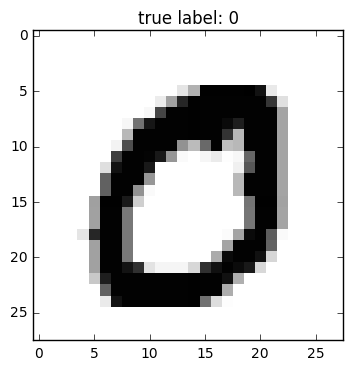
\includegraphics[width=0.1\textwidth]{../img/delaunay_new/mnist_data_0.png}
{\huge $\qquad \xrightarrow{\quad f \quad} \qquad 0$}
\end{center}

\bigskip
$$
28 \times 28 \text{ pixels} \neq 784 \text{ dimensions...}
$$
\end{frame}

\begin{frame}
\frametitle{The curse of dimensionality}

\begin{columns}
\begin{column}{0.5\textwidth}
\begin{center}
\includegraphics[width=0.8\textwidth]{../img/delaunay_new/inference_2d_pt1.eps}\\
10 training points in 1D
\end{center}
\end{column}

\begin{column}{0.5\textwidth}
\begin{center}
\includegraphics[width=0.95\textwidth]{../img/delaunay_new/inference_2d_pt2.eps}\\
10 training points in 2D
\end{center}
\end{column}
\end{columns}
\end{frame}

\begin{frame}
\frametitle{The curse of \sout{dimensionality} no data}

\begin{columns}
\begin{column}{0.5\textwidth}
\begin{center}
\includegraphics[width=0.8\textwidth]{../img/delaunay_new/inference_2d_pt3.eps}\\
Need data in all quadrants?
\end{center}
\end{column}

\begin{column}{0.5\textwidth}
\pause
\begin{itemize}
\item Inference in 2D : $2^2 = 4$
\item Inference in 10D : $2^{10} \approx 1000$
\item Inference in 100D : $2^{100} \approx 10^{30}$ (orders of magnitude bigger than exascale)
\item Many ML problems : inference in 1000+ dimensions
\end{itemize}
\end{column}
\end{columns}

\end{frame}

%\begin{frame}
%\frametitle{The blessing of dimensionality (no noise)}
%
%\begin{center}
%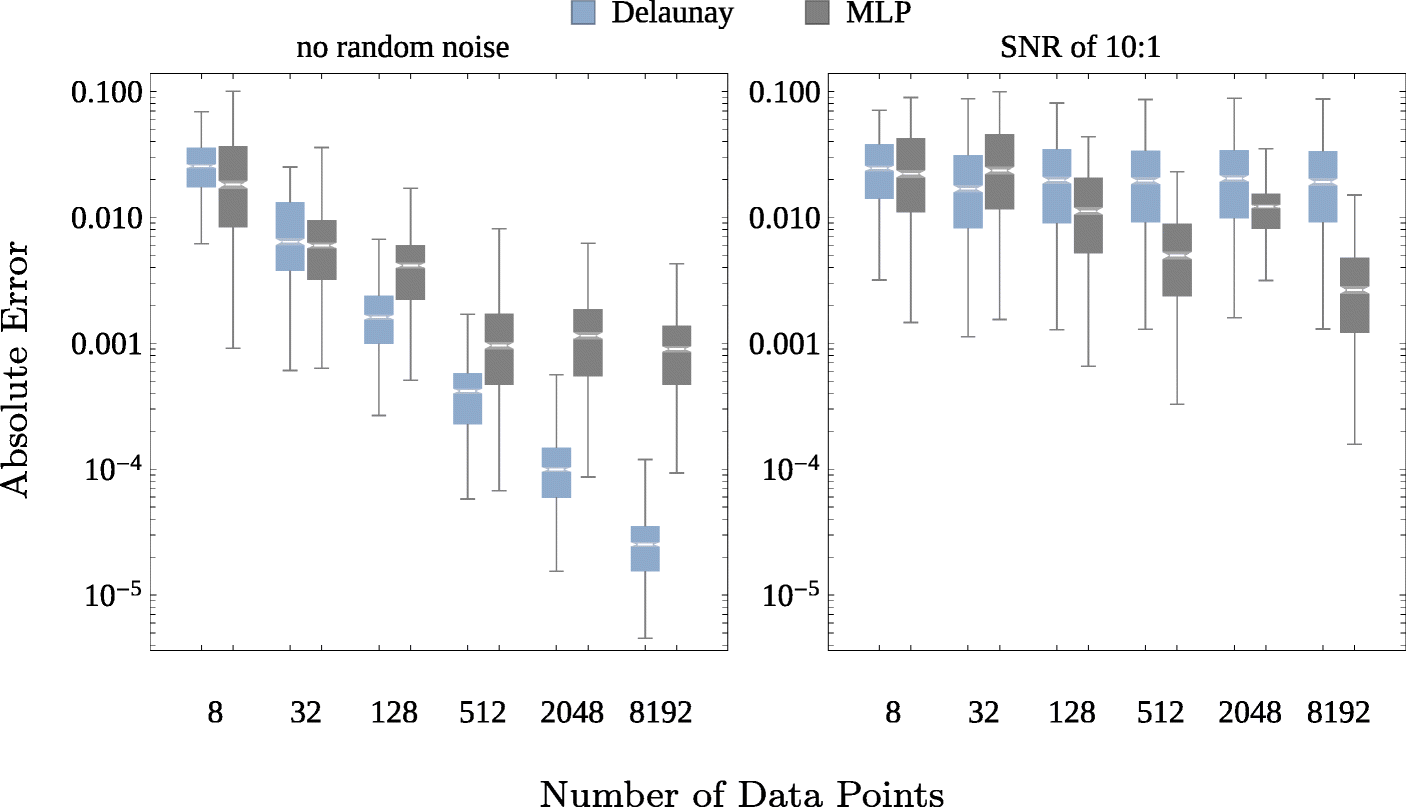
\includegraphics[width=0.7\textwidth]{../img/delaunay_new/2d_errors_w_noise.png}\\
%Delaunay interpolation vs MLP error in {\bf 2D} with and w/o noise
%\end{center}
%
%\vfill
%
%{\tiny Lux, Watson, Chang, et al.
%Interpolation of sparse high-dimensional data.
%{\sl Numerical Algorithms 88}, pp.~281–313 (2021).}
%
%\end{frame}
%
%\begin{frame}
%\frametitle{The blessing of dimensionality (no noise)}
%
%\begin{center}
%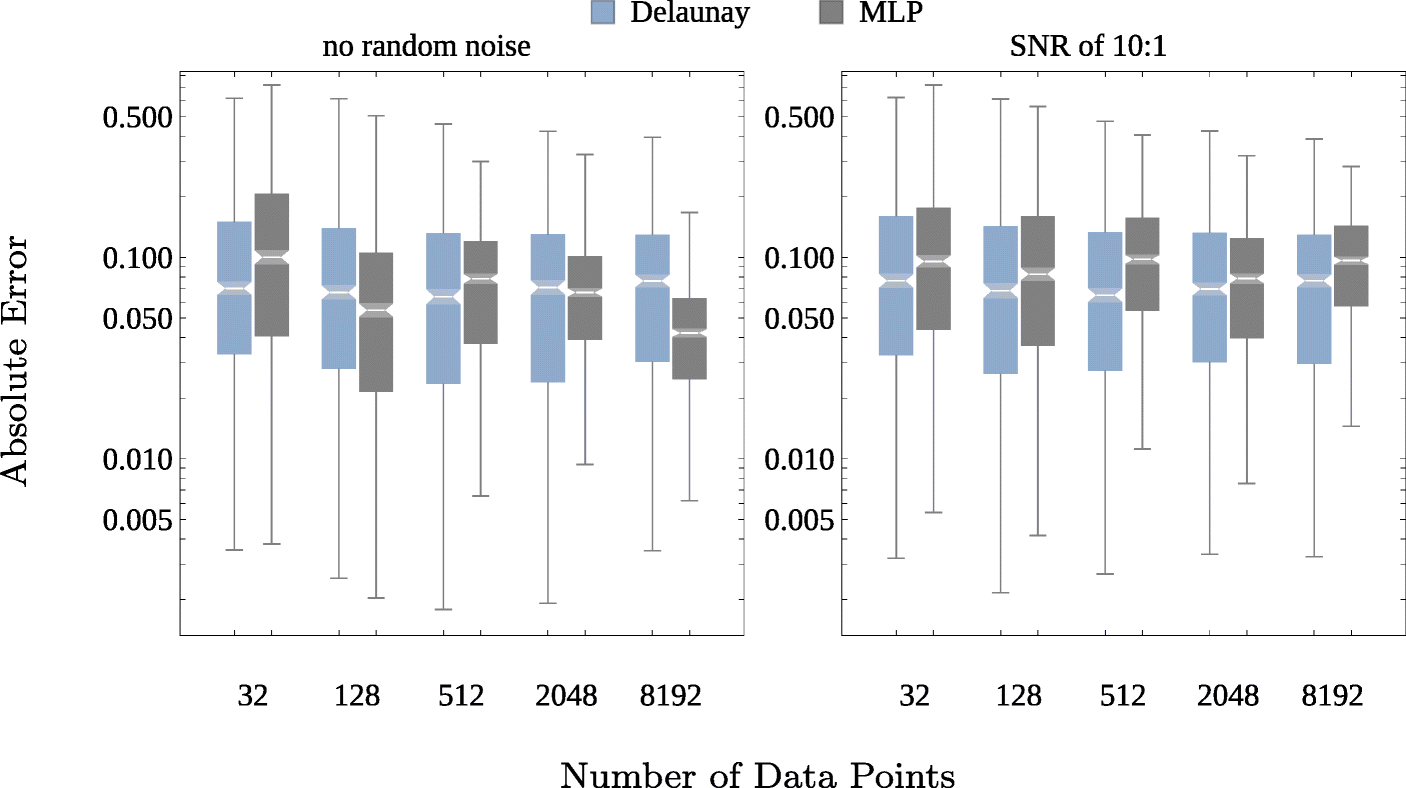
\includegraphics[width=0.7\textwidth]{../img/delaunay_new/20d_errors_w_noise.png}\\
%Delaunay interpolation vs MLP error in {\bf 20D} with and w/o noise
%\end{center}
%
%\vfill
%
%{\tiny Lux, Watson, Chang, et al.,
%Interpolation of sparse high-dimensional data.
%{\sl Numerical Algorithms 88}, pp.~281–313 (2021).}
%
%\end{frame}

\begin{frame}
\frametitle{Measure collapse}

Can we still make good predictions where we {\bf do} have data?

\bigskip
\pause

{\bf No, because we have no data anywhere}

\bigskip

We measure where we {\sl might} have enough data to make a prediction
using the ``convex hull'' of the training data $CH({\cal X})$

\bigskip
\pause

If ${\cal X}$ are sampled from {\sl any} distribution,
$\mu(CH({\cal X})) \rightarrow 0$ {\sl exponentially} as $d$ grows

\bigskip

This is called a {\sl concentration of measure}

\vfill

{\tiny Gorban and Tyukin,
Stochastic separation theorems.
{\sl Neural Networks 94}, pp.~255-259 (2017).}

\end{frame}

\begin{frame}
\frametitle{Example}

Suppose that we uniformly sample $x = (x_1, x_2, \ldots, x_d)$ from $[0, 1]^d$

\bigskip

$$
\|x - \frac{1}{2}\|_2^2 = \sum_{i=1}^d{(x_i - \frac{1}{2})^2}.
$$

$$
\mathbb{E}\left[ \left(x_i - \frac{1}{2}\right)^2 \right]
= \int_{0}^1 \left(u - \frac{1}{2}\right)^2 du
= \frac{1}{12}
$$
with finite variance $\nu$

\bigskip

By CLT for all $x \in {\cal X}$:
$\mathbb{E}[\|x - \frac{1}{2}\|_2^2] = \frac{d}{12}$
with variance $\frac{\nu}{d}\rightarrow 0$ as $d\rightarrow\infty$.

\end{frame}

\begin{frame}
\frametitle{Collapse of some common distributions}

\begin{center}
\includegraphics[width=0.45\textwidth]{../img/moo_new/discrep_linear.eps}
\includegraphics[width=0.45\textwidth]{../img/moo_new/discrep_log.eps}
\end{center}

\vfill

{\tiny Garg, Chang, and Raghavan,
Stochastic optimization of Fourier coefficiencts to generate space-filling designs.
{\sl To appear in Winter Sim 2023}.}

\end{frame}

\begin{frame}
\frametitle{Modern deep learning pipeline}

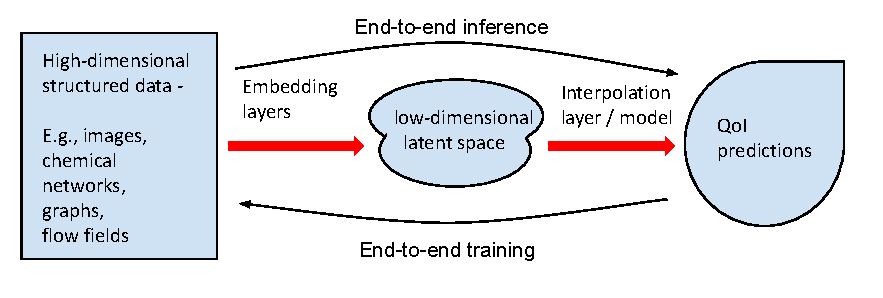
\includegraphics{../img/delaunay_new/interpolating_latent_space.pdf}

\end{frame}

\section{Modeling for high-dimensional optimization}

\begin{frame}
\frametitle{Hope in context of optimization}

\begin{center}
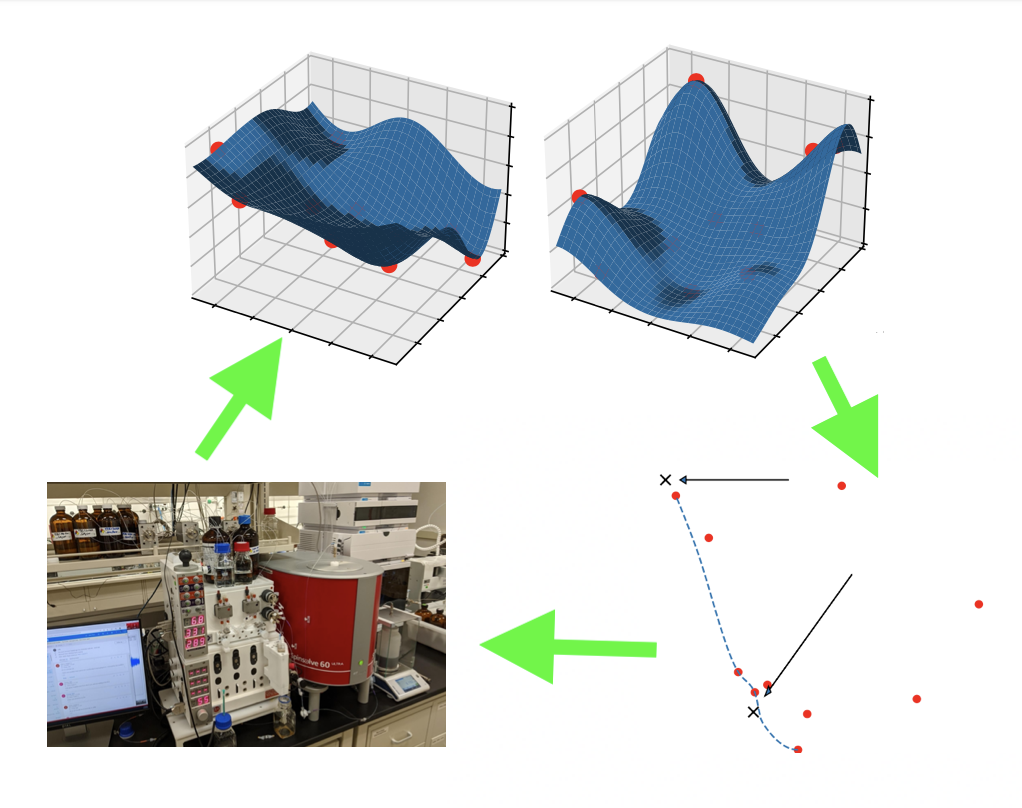
\includegraphics[width=0.55\textwidth]{../img/moo_new/iclr-thumbnail.png}
\end{center}

\end{frame}

\begin{frame}
\frametitle{Global modeling is harder than optimization}

For optimization, only need model accuracy near the solution...

\begin{itemize}
\item Global modeling is {\sl significantly harder than optimizing}
\item To build a {\sl globally accurate model} over $n$ variables, need ${\cal O}(2^n)$ samples
\item To build a {\sl locally accurate model} over $n$ variables, need ${\cal O}(n)$ samples
\end{itemize}
\end{frame}

\begin{frame}
\frametitle{Global optimization}
In global optimization literature...
\begin{itemize}
\item Balance exploration vs.\ exploitation
\item Drive {\sl global model error} to zero
\item Need exponentially many samples to guarantee global convergence
\end{itemize}

Guarantees convergence for problems with thousands of local minima

\begin{center}
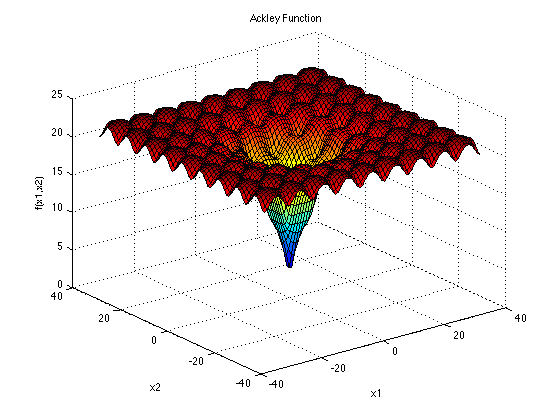
\includegraphics[width=0.35\textwidth]{../img/moo_new/ackley.png}
$\qquad\qquad$
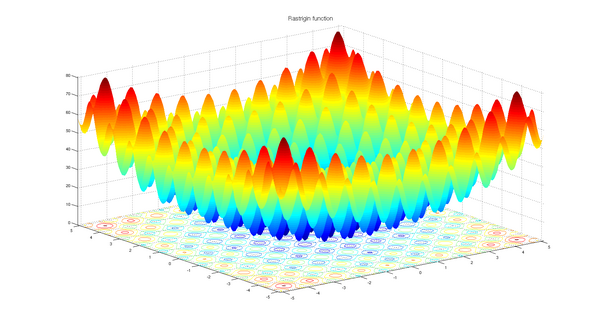
\includegraphics[width=0.4\textwidth]{../img/moo_new/rastrigin.png}
\end{center}

\end{frame}

\end{document}
